\documentclass[12pt,a4paper,twoside]{report}

% ---- Encodage et langue ----
\usepackage[french]{babel}
\usepackage[T1]{fontenc}
\usepackage[utf8]{inputenc}
\usepackage{lmodern}

% ---- Géométrie ----
\usepackage{geometry}
\geometry{
  top=2.5cm,
  bottom=2.5cm,
  left=3cm,
  right=2.5cm,
  bindingoffset=0.5cm
}

% ---- Packages ----
\usepackage{graphicx}
\usepackage{hyperref}
\usepackage{enumitem}
\usepackage{listings}
\usepackage{xcolor}
\usepackage{booktabs}
\usepackage{longtable}
\usepackage{array}
\usepackage{float}
\usepackage{caption}
\usepackage{subcaption}
\usepackage{amsmath}
\usepackage{amssymb}
\usepackage{multirow}
\usepackage{setspace}
\usepackage{titlesec}
\usepackage{fancyhdr}
\usepackage{cite}
\usepackage{tocloft}
\usepackage{appendix}

% ---- Couleurs et style ----
\definecolor{codegreen}{rgb}{0,0.6,0}
\definecolor{codegray}{rgb}{0.5,0.5,0.5}
\definecolor{codepurple}{rgb}{0.58,0,0.82}
\definecolor{backcolour}{rgb}{0.95,0.95,0.92}

\lstdefinestyle{mystyle}{
  backgroundcolor=\color{backcolour},
  commentstyle=\color{codegreen},
  keywordstyle=\color{magenta},
  numberstyle=\tiny\color{codegray},
  stringstyle=\color{codepurple},
  basicstyle=\ttfamily\footnotesize,
  breakatwhitespace=false,
  breaklines=true,
  captionpos=b,
  keepspaces=true,
  numbers=left,
  numbersep=5pt,
  showspaces=false,
  showstringspaces=false,
  showtabs=false,
  tabsize=2
}
\lstset{style=mystyle}

% ---- En-têtes et pieds de page ----
\pagestyle{fancy}
\fancyhf{}
\fancyhead[LE,RO]{\thepage}
\fancyhead[RE]{\leftmark}
\fancyhead[LO]{\rightmark}
\renewcommand{\headrulewidth}{0.4pt}

% ---- Espacement ----
\onehalfspacing

% ---- Info document ----
\title{
  \vspace*{3cm}
  \Huge\textbf{Détection de la Pneumonie sur Radiographies Thoraciques}\\[0.8cm]
  \Large\textbf{par Apprentissage Profond :}\\[0.3cm]
  \Large{De la Classification à la Segmentation avec U-Net}\\[2cm]
  \vspace*{1cm}
}
\author{
  \textbf{Issam Sensi}\\[0.3cm]
  \texttt{issam.sensi@example.com}\\[1cm]
  \large{Rapport de Projet -- Master}\\[0.3cm]
  \large{Année universitaire 2025--2026}
}
\date{\today}

\begin{document}

% ============== PAGE DE GARDE ==============
\begin{titlepage}
\centering
\vspace*{2cm}

\rule{\textwidth}{1pt}\\[0.3cm]
{\Huge\textbf{Détection de la Pneumonie\\[0.3cm] sur Radiographies Thoraciques\\[0.3cm] par Apprentissage Profond}}\\[0.3cm]
\rule{\textwidth}{1pt}\\[0.8cm]

{\large De la Classification à la Segmentation avec U-Net}\\[1.5cm]

\vspace*{2cm}

{\large\textbf{Issam Sensi}}\\[0.3cm]
{\large\texttt{issam.sensi@example.com}}\\[1.5cm]

{\large Rapport de Projet}\\[0.3cm]
{\large Master en Intelligence Artificielle}\\[0.3cm]
{\large Année universitaire 2025--2026}\\[2cm]

\vfill
\end{titlepage}

% ============== RÉSUMÉ ==============
\chapter*{Résumé}
\addcontentsline{toc}{chapter}{Résumé}

Ce rapport présente le développement d'un outil de détection de la pneumonie à partir de radiographies thoraciques, basé sur l'apprentissage profond. La pneumonie est une infection pulmonaire grave qui reste l'une des principales causes de mortalité dans le monde. Le diagnostic repose sur l'interprétation de radiographies par des radiologues, un processus qui peut être subjectif et sujet à des variations inter-opérateurs.

Plusieurs architectures de deep learning ont été explorées et comparées :
\begin{itemize}
  \item \textbf{DenseNet121 et MobileNet} : classifieurs binaires pré-entraînés, rapides mais ne fournissant aucune information spatiale sur la localisation des lésions.
  \item \textbf{YOLOv8} : détecteur d'objets par boîtes englobantes, abandonné en raison d'une précision insuffisante, d'un temps d'entraînement long et de la nécessité d'utiliser Grad-CAM pour la visualisation.
  \item \textbf{U-Net résiduelle} : architecture de segmentation pixel-level avec tête de classification intégrée, retenue comme solution finale.
\end{itemize}

Le modèle U-Net atteint des performances solides avec un IoU de 0,71 pour la segmentation, une précision de classification de 93\,\%, un AUROC de 0,98, un rappel de 89\,\% et un F1-score de 91\,\%. Le masque de segmentation sert directement de carte de chaleur, éliminant le besoin de techniques de visualisation séparées comme Grad-CAM.

L'application web développée avec Flask permet de télécharger une radiographie, d'obtenir un diagnostic avec une carte de chambre superposée et de générer un rapport PDF. Ce projet constitue une démonstration fonctionnelle d'un pipeline complet de deep learning pour l'imagerie médicale, de l'entraînement du modèle à l'interface utilisateur.

\vspace{0.5cm}
\textbf{Mots-clés :} Deep learning, U-Net, segmentation sémantique, pneumonie, radiographie thoracique, RSNA, TensorFlow, Flask, interprétabilité.

% ============== REMERCIEMENTS ==============
\chapter*{Remerciements}
\addcontentsline{toc}{chapter}{Remerciements}

Je tiens à exprimer ma gratitude envers toutes les personnes qui ont contribué à la réalisation de ce projet.

Je remercie particulièrement l'équipe pédagogique du Master pour m'avoir fourni les connaissances théoriques et pratiques nécessaires à ce travail. La Radiological Society of North America (RSNA) mérite une mention spéciale pour avoir mis à disposition le dataset de radiographies thoraciques qui a servi de base à cette étude.

Je remercie également la communauté open source pour les outils et bibliothèques utilisés dans ce projet : TensorFlow, Keras, Flask, OpenCV, et bien d'autres.

Enfin, un grand merci à ma famille et à mes proches pour leur soutien tout au long de ce travail.
\newpage
\tableofcontents
\newpage

% ================================================================
% CHAPITRE 1 — INTRODUCTION
% ================================================================
\chapter{Introduction}

\section{Contexte médical}

La pneumonie est une infection respiratoire aiguë qui affecte les alvéoles pulmonaires. Selon l'Organisation Mondiale de la Santé (OMS), la pneumonie est responsable d'environ 700\,000 décès par an chez les enfants de moins de cinq ans, ce qui en fait la première cause infectieuse de mortalité infantile dans le monde \cite{who-pneumonia}. Chez les adultes, particulièrement les personnes âgées et les immunodéprimés, la pneumonie représente également un danger majeur.

Le diagnostic de la pneumonie repose généralement sur une combinaison d'examens cliniques, d'analyses biologiques et d'imagerie médicale. La radiographie thoracique (ou \textit{chest X-ray}) est l'examen d'imagerie le plus couramment utilisé en raison de sa rapidité, de son faible coût et de sa disponibilité généralisée. Sur une radiographie, les poumons sains apparaissent sombres (remplis d'air), tandis que les zones infectées par la pneumonie se manifestent par des opacités de formes et de tailles variables, allant du gris au blanc.

L'interprétation des radiographies thoraciques est un exercice complexe qui nécessite une formation spécialisée. Plusieurs facteurs rendent cette tâche difficile :
\begin{itemize}
  \item La superposition d'organes (cœur, diaphragme, côtes) peut masquer des zones d'opacité.
  \item La variabilité anatomique inter-patients liée à l'âge, au sexe et à la morphologie.
  \item La nature hétérogène de la pneumonie elle-même, qui peut affecter différentes zones avec des apparences radiologiques variées.
\end{itemize}

Ces défis entraînent une variabilité inter-opérateur significative et soulignent le besoin d'outils d'aide au diagnostic assisté par ordinateur.

\section{Apprentissage profond pour l'imagerie médicale}

L'apprentissage profond (\textit{deep learning}) a révolutionné le domaine de la vision par ordinateur au cours de la dernière décennie. Dans le domaine médical, les réseaux de neurones convolutifs (CNN) ont démontré des performances remarquables pour diverses tâches : classification de pathologies, segmentation d'organes, détection de lésions, etc.

Plusieurs approches sont possibles pour l'analyse d'images médicales :

\begin{itemize}
  \item \textbf{Classification} : l'image est assignée à une classe (normal / pathologique). Simple et rapide, mais ne fournit pas d'information spatiale.
  \item \textbf{Détection d'objets} : des boîtes englobantes localisent les régions d'intérêt. Plus informative que la classification, mais limitée par la forme rectangulaire des boîtes.
  \item \textbf{Segmentation sémantique} : chaque pixel de l'image est classifié, produisant un masque détaillé. C'est l'approche la plus informative et la plus naturelle pour l'imagerie médicale.
\end{itemize}

\section{Objectifs du projet}

Ce projet vise à développer un pipeline complet de détection de la pneumonie sur radiographies thoraciques, avec les objectifs suivants :

\begin{enumerate}
  \item Explorer et comparer différentes architectures de deep learning pour cette tâche.
  \item Développer un modèle capable de fournir à la fois un diagnostic et une visualisation interprétable.
  \item Déployer le modèle dans une application web fonctionnelle avec interface utilisateur.
  \item Permettre la génération de rapports PDF exportables.
\end{enumerate}

\section{Structure du rapport}

Ce rapport est organisé comme suit :
\begin{itemize}
  \item Le \textbf{Chapitre 2} présente l'état de l'art et les travaux connexes.
  \item Le \textbf{Chapitre 3} décrit le dataset utilisé et les prétraitements appliqués.
  \item Le \textbf{Chapitre 4} détaille les différentes architectures explorées.
  \item Le \textbf{Chapitre 5} présente la méthodologie d'entraînement.
  \item Le \textbf{Chapitre 6} analyse les résultats obtenus.
  \item Le \textbf{Chapitre 7} décrit l'application web développée.
  \item Le \textbf{Chapitre 8} conclut et propose des perspectives.
\end{itemize}

% ================================================================
% CHAPITRE 2 — ÉTAT DE L'ART
% ================================================================
\chapter{État de l'Art}

\section{Introduction}

La détection automatisée de la pneumonie à partir de radiographies thoraciques est un domaine de recherche actif depuis plusieurs années. Avec l'avènement du deep learning, de nombreuses architectures ont été proposées, allant des classifieurs simples aux modèles de segmentation complexes.

\section{Approches par classification}

Les réseaux de neurones convolutifs pré-entraînés sur ImageNet constituent une approche courante pour la classification d'images médicales. Des architectures comme DenseNet \cite{densenet} et MobileNet \cite{mobilenet} ont été largement utilisées :

\begin{itemize}
  \item \textbf{DenseNet121} : introduit des connexions denses entre toutes les couches, chaque couche recevant en entrée les feature maps de toutes les couches précédentes. Cela permet une meilleure circulation du gradient et une réutilisation des caractéristiques. DenseNet a été utilisé avec succès sur le dataset ChestX-ray14 pour la détection de pathologies thoraciques \cite{wang2017chestx-ray14}.
  
  \item \textbf{MobileNet} : conçu pour les environnements à ressources limitées, il utilise des convolutions depthwise séparables pour réduire le nombre de paramètres et le coût computationnel tout en maintenant des performances compétitives.
\end{itemize}

Cependant, ces approches présentent une limitation fondamentale : elles ne fournissent que la probabilité d'appartenance à une classe, sans aucune information sur la localisation des anomalies dans l'image. Pour un clinicien, savoir \textit{où} se trouve l'anomalie est aussi important que de savoir \textit{si} elle est présente.

\section{Approches par détection d'objets}

Les détecteurs d'objets comme YOLO (You Only Look Once) \cite{yolo} permettent de localiser les anomalies à l'aide de boîtes englobantes. YOLOv8 \cite{ultralytics} est la dernière itération de cette famille de modèles, offrant un bon compromis entre précision et rapidité.

Avantages :
\begin{itemize}
  \item Localisation approximative des lésions via des boîtes englobantes.
  \item Inférence rapide, adaptée au temps réel.
\end{itemize}

Inconvénients :
\begin{itemize}
  \item Les boîtes englobantes sont trop grossières pour des lésions diffuses ou de forme irrégulière.
  \item L'entraînement nécessite des annotations sous forme de boîtes, qui ne sont pas toujours disponibles.
  \item Difficulté à modéliser la confiance pour la classe « normale » (absence de boîte).
\end{itemize}

\section{Approches par segmentation}

La segmentation sémantique est l'approche la plus naturelle pour l'imagerie médicale. U-Net \cite{unet} est l'architecture de référence dans ce domaine, conçue spécifiquement pour la segmentation d'images biomédicales.

U-Net se caractérise par :
\begin{itemize}
  \item Une architecture en forme de « U » avec un encodeur (contraction) et un décodeur (expansion) symétriques.
  \item Des connexions de saut (\textit{skip connections}) entre les niveaux correspondants de l'encodeur et du décodeur, permettant de préserver les informations spatiales fines.
  \item Une capacité à produire des segmentations précises même avec peu de données d'entraînement.
\end{itemize}

Depuis sa publication en 2015, U-Net a connu de nombreuses variantes : U-Net avec blocs résiduels (ResUNet), U-Net avec attention (Attention U-Net), U-Net 3D pour les volumes médicaux, etc.

\section{Interprétabilité en imagerie médicale}

L'interprétabilité des modèles de deep learning est cruciale dans le domaine médical. Plusieurs techniques ont été développées :

\begin{itemize}
  \item \textbf{Grad-CAM} \cite{gradcam} : utilise les gradients de la dernière couche convolutive pour produire une carte de chaleur. Simple à implémenter mais nécessite une passe arrière supplémentaire et peut être instable.
  \item \textbf{Saliency maps} : calculent l'impact de chaque pixel sur la prédiction.
  \item \textbf{LIME} : explique les prédictions en approximant localement le modèle par un modèle interprétable.
\end{itemize}

La segmentation sémantique offre un avantage naturel pour l'interprétabilité : le masque de segmentation constitue en lui-même une carte de chaleur intrinsèque, éliminant le besoin de techniques de post-hoc.

\section{Positionnement du projet}

Ce projet se positionne à l'intersection de ces différentes approches. En combinant segmentation et classification dans un modèle unique (U-Net hybride), nous bénéficions :
\begin{itemize}
  \item De la précision spatiale de la segmentation.
  \item De la simplicité d'interprétation d'un masque pixel-level.
  \item De la fiabilité d'une tête de classification dédiée pour le verdict binaire.
\end{itemize}

% ================================================================
% CHAPITRE 3 — DATASET
% ================================================================
\chapter{Dataset et Prétraitement}

\section{Le dataset RSNA Pneumonia Challenge}

Le dataset utilisé dans ce projet provient du \textbf{RSNA Pneumonia Detection Challenge}, une compétition organisée en 2018 par la Radiological Society of North America (RSNA) en collaboration avec la National Institutes of Health (NIH) et d'autres institutions \cite{rsna2018}.

\subsection{Description}

Le dataset original contient 26\,684 radiographies thoraciques au format DICOM, annotées par des radiologues certifiés. Les annotations se présentent sous deux formes :
\begin{itemize}
  \item Des \textbf{boîtes englobantes} (bounding boxes) délimitant les zones d'opacité pour les cas de pneumonie.
  \item Une \textbf{étiquette binaire} (Target) : 0 pour normal, 1 pour pneumonie.
\end{itemize}

\subsection{Dataset prétraité}

Pour ce projet, nous utilisons une version prétraitée du dataset RSNA, disponible sur Kaggle sous le nom \textit{« RSNA Pneumonia Processed Dataset »}. Ce dataset convertit les boîtes englobantes originales en \textbf{masques de segmentation pixel-level}, facilitant l'utilisation d'architectures de segmentation comme U-Net.

\subsection{Structure des données}

\begin{verbatim}
/kaggle/input/rsna-pneumonia-processed-dataset/
  |-- stage2_train_metadata.csv     # Métadonnées d'entraînement
  |-- stage2_test_metadata.csv      # Métadonnées de test
  |-- Training/
  |     |-- Images/                 # 26 684 radiographies (PNG)
  |     |-- Masks/                  # 26 684 masques (PNG)
  |-- Test/
        |-- Images/
        |-- Masks/
\end{verbatim}

\subsection{Métadonnées}

Le fichier CSV contient les colonnes suivantes :

\begin{table}[H]
\centering
\begin{tabular}{lll}
\toprule
\textbf{Colonne} & \textbf{Type} & \textbf{Description} \\
\midrule
\texttt{patientId} & chaîne & Identifiant unique du patient \\
\texttt{age} & numérique & Âge du patient \\
\texttt{sex} & catégoriel & M (masculin) / F (féminin) \\
\texttt{position} & catégoriel & AP (antéropostérieure) / PA (postéroantérieure) \\
\texttt{class} & chaîne & Lung Opacity / Normal \\
\texttt{Target} & binaire & 0 (normal) / 1 (pneumonie) \\
\bottomrule
\end{tabular}
\caption{Description des colonnes du fichier de métadonnées}
\end{table}

\section{Analyse exploratoire}

\subsection{Distribution des classes}

Le dataset présente un déséquilibre de classes, avec une majorité de cas normaux par rapport aux cas de pneumonie. Cette distribution est naturelle dans un contexte clinique où la prévalence de la pneumonie dans la population générale est relativement faible.

\begin{figure}[H]
\centering
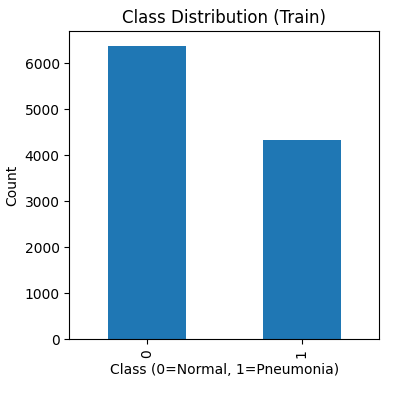
\includegraphics[width=0.6\textwidth]{images/class_distribution.png}
\caption{Distribution des classes dans le dataset}
\end{figure}

Ce déséquilibre est pris en compte lors de l'entraînement via l'utilisation de poids de classe (\textit{class weights}) dans la fonction de perte.

\subsection{Visualisation des données}

Les radiographies thoraciques sont des images en niveaux de gris de résolution variable. Les poumons sains apparaissent sombres (radio-transparents), tandis que les zones d'opacité caractéristiques de la pneumonie apparaissent en blanc/gris.

Les masques de segmentation correspondants sont binaires : fond noir (0) pour les pixels sains, blanc (1) pour les pixels pathologiques.

\section{Prétraitement des données}

\subsection{Prétraitement des images}

Le pipeline de prétraitement des images comprend les étapes suivantes :

\begin{enumerate}
  \item \textbf{Chargement} : lecture du fichier PNG avec TensorFlow.
  \item \textbf{Redimensionnement} : à 224$\times$224 pixels (format d'entrée du modèle U-Net).
  \item \textbf{Normalisation} : mise à l'échelle des valeurs des pixels dans l'intervalle $[0, 1]$ par division par 255.
  \item \textbf{Augmentation} (entraînement uniquement) : variation aléatoire de la luminosité ($\delta = 0,1$) et du contraste ($[0,9, 1,1]$).
\end{enumerate}

\subsection{Prétraitement des masques}

\begin{enumerate}
  \item Chargement du fichier PNG du masque.
  \item Redimensionnement à 224$\times$224.
  \item Binarisation : toute valeur $>0$ est convertie en 1.
\end{enumerate}

\subsection{Prétraitement des données tabulaires}

Les caractéristiques démographiques des patients sont également utilisées par le modèle :

\begin{itemize}
  \item \textbf{Sexe} : encodage binaire (M $\rightarrow$ 0, F $\rightarrow$ 1).
  \item \textbf{Position} : encodage binaire (AP $\rightarrow$ 0, PA $\rightarrow$ 1).
  \item \textbf{Âge} : plafonnement à 90 ans, puis normalisation MinMax dans $[0, 1]$.
\end{itemize}

\subsection{Pipeline de données tf.data}

Pour l'entraînement, nous utilisons l'API \texttt{tf.data} de TensorFlow qui permet de construire des pipelines de données efficaces et parallélisées :

\begin{itemize}
  \item \textbf{Chargement asynchrone} : les images sont chargées et prétraitées en parallèle du calcul sur GPU.
  \item \textbf{Shuffle} : mélange aléatoire des échantillons à chaque époque.
  \item \textbf{Batching} : regroupement par lots de 64 échantillons.
  \item \textbf{Prefetch} : préchargement du lot suivant pendant le calcul du lot courant.
\end{itemize}

\subsection{Division du dataset}

Le dataset est divisé en trois sous-ensembles :

\begin{table}[H]
\centering
\begin{tabular}{lcc}
\toprule
\textbf{Ensemble} & \textbf{Proportion} & \textbf{Échantillons} \\
\midrule
Entraînement & 72\,\% & $\sim$19\,200 \\
Validation & 8\,\% & $\sim$2\,130 \\
Test & 10\,\% & $\sim$2\,670 \\
\bottomrule
\end{tabular}
\caption{Division du dataset}
\end{table}

La division est stratifiée sur la variable \texttt{Target} afin de préserver la proportion de classes dans chaque sous-ensemble.

% ================================================================
% CHAPITRE 4 — ARCHITECTURES EXPLORÉES
% ================================================================
\chapter{Architectures Explorées}

\section{Introduction}

Ce chapitre présente les différentes architectures de deep learning explorées dans le cadre de ce projet. Chaque architecture est évaluée selon plusieurs critères : précision, vitesse d'entraînement, capacité de localisation et interprétabilité.

\section{DenseNet121}

\subsection{Architecture}

DenseNet121 \cite{densenet} est un réseau de neurones convolutif profond introduit par Huang et al. en 2017. Son innovation principale est le \textit{dense connectivity pattern} : chaque couche reçoit en entrée les feature maps de toutes les couches précédentes et transmet ses propres feature maps à toutes les couches suivantes.

Pour un réseau à $L$ couches, le nombre de connexions est de $\frac{L(L+1)}{2}$, contre $L$ pour un réseau conventionnel.

\subsection{Avantages}
\begin{itemize}
  \item Atténuation du problème de vanishing gradient grâce aux connexions denses.
  \item Réutilisation des caractéristiques à différents niveaux d'abstraction.
  \item Nombre de paramètres relativement faible comparé à d'autres architectures profondes.
\end{itemize}

\subsection{Inconvénients}
\begin{itemize}
  \item Classification uniquement : aucune information spatiale.
  \item Impossible de localiser les lésions dans l'image.
\end{itemize}

\section{MobileNet}

\subsection{Architecture}

MobileNet \cite{mobilenet} a été conçu par Howard et al. (2017) pour les applications mobiles et embarquées. Son innovation clé est l'utilisation de \textit{depthwise separable convolutions}, qui factorisent une convolution standard en deux étapes :
\begin{enumerate}
  \item Une convolution depthwise (appliquée à chaque canal indépendamment).
  \item Une convolution pointwise (convolution 1$\times$1 pour combiner les canaux).
\end{enumerate}

Cette factorisation réduit considérablement le nombre d'opérations et la taille du modèle.

\subsection{Avantages}
\begin{itemize}
  \item Modèle très compact et rapide.
  \item Adapté au déploiement sur des ressources limitées.
\end{itemize}

\subsection{Inconvénients}
\begin{itemize}
  \item Même limitation que DenseNet : classification sans localisation.
  \item Précision légèrement inférieure à des modèles plus profonds.
\end{itemize}

\section{YOLOv8}

\subsection{Architecture}

YOLO (You Only Look Once) \cite{yolo} est une famille de modèles de détection d'objets qui traite la détection comme un problème de régression. YOLOv8 \cite{ultralytics}, développé par Ultralytics, est la dernière version de cette architecture.

L'architecture YOLOv8 se compose de trois parties principales :
\begin{enumerate}
  \item Un \textbf{backbone} (CSPDarknet) pour l'extraction de caractéristiques.
  \item Un \textbf{neck} (PAN-FPN) pour la fusion des caractéristiques multi-échelles.
  \item Une \textbf{tête de détection} qui prédit les boîtes englobantes et les classes.
\end{enumerate}

\subsection{Problèmes rencontrés}

\subsubsection{Précision insuffisante}
Le modèle YOLO a montré des difficultés à converger vers une solution satisfaisante. La perte d'entraînement restait élevée et la précision sur l'ensemble de validation était insuffisante.

\subsubsection{Temps d'entraînement long}
Avec environ 11 millions de paramètres et une taille d'entrée de 640$\times$640 pixels, chaque époque d'entraînement prenait un temps considérable, même sur GPU.

\subsubsection{Confiance pour la classe « normale »}
La confiance pour un diagnostic de « normal » était calculée heuristiquement comme $1 - \text{confiance\_max\_des\_boîtes}$, une approximation peu fiable.

\subsubsection{Localisation imprécise}
Les boîtes englobantes sont trop grossières pour des lésions diffuses ou de forme irrégulière, ce qui est souvent le cas des opacités pneumoniques.

\subsubsection{Grad-CAM instable}
La visualisation par Grad-CAM nécessitait des hooks sur les gradients et une passe arrière supplémentaire, avec des problèmes de buffers détachés sur le modèle YOLO d'Ultralytics.

\section{U-Net Résiduelle}

\subsection{Architecture}

L'U-Net \cite{unet}, introduite par Ronneberger et al. (2015), est l'architecture de référence pour la segmentation d'images biomédicales. Notre implémentation intègre des blocs résiduels et une fusion de données tabulaires.

\subsubsection{Encodeur}

L'encodeur suit une structure hiérarchique à 4 niveaux, chaque niveau réduisant la résolution spatiale de moitié tout en doublant le nombre de filtres :

\begin{table}[H]
\centering
\begin{tabular}{lccc}
\toprule
\textbf{Niveau} & \textbf{Filtres} & \textbf{Résolution} & \textbf{Sortie} \\
\midrule
Entrée & 3 & 224$\times$224 & Image RGB \\
Niveau 1 & 32 & 224$\times$224 & Conv + Bloc résiduel \\
Niveau 2 & 64 & 112$\times$112 & Conv + Bloc résiduel \\
Niveau 3 & 128 & 56$\times$56 & Conv + Bloc résiduel \\
Niveau 4 & 256 & 28$\times$28 & Conv + Bloc résiduel \\
Goulot & 512 & 14$\times$14 & Conv + Dropout 0.3 \\
\bottomrule
\end{tabular}
\caption{Architecture de l'encodeur}
\end{table}

\subsubsection{Décodeur}

Le décodeur symétrique utilise des convolutions transposées pour augmenter la résolution :

\begin{table}[H]
\centering
\begin{tabular}{lccc}
\toprule
\textbf{Niveau} & \textbf{Filtres} & \textbf{Concaténation} & \textbf{Sortie} \\
\midrule
Niveau 4 & 256 & Avec encodeur niveau 4 & 28$\times$28 \\
Niveau 3 & 128 & Avec encodeur niveau 3 & 56$\times$56 \\
Niveau 2 & 64 & Avec encodeur niveau 2 & 112$\times$112 \\
Niveau 1 & 32 & Avec encodeur niveau 1 & 224$\times$224 \\
\bottomrule
\end{tabular}
\caption{Architecture du décodeur}
\end{table}

\subsubsection{Fusion tabulaire}

Les caractéristiques tabulaires (âge, sexe, position) sont traitées par une couche dense de 64 neurones, puis redimensionnées à 224$\times$224 et concaténées avec les caractéristiques du décodeur.

\subsubsection{Sorties}

Le modèle produit deux sorties :
\begin{enumerate}
  \item \textbf{Masque de segmentation} : couche Conv2D 1$\times$1 avec activation sigmoïde, produisant une carte de probabilités de 224$\times$224 pixels.
  \item \textbf{Classification binaire} : GlobalAveragePooling, couche dense de 64 neurones, puis couche dense finale avec activation sigmoïde.
\end{enumerate}

\subsection{Blocs résiduels}

Chaque bloc résiduel de l'architecture s'écrit :

\begin{equation}
\mathbf{y} = \sigma(\mathbf{x} + \mathcal{F}(\mathbf{x}, W_i))
\end{equation}

où $\mathcal{F}$ représente deux convolutions 3$\times$3 avec normalisation par lot et activation LeakyReLU, et $\sigma$ est la fonction d'activation LeakyReLU finale.

\subsection{Fonctions de perte}

\subsubsection{Pour le masque : IoU Loss}

La perte IoU (Intersection over Union) est définie par :

\begin{equation}
\mathcal{L}_{\text{mask}} = 1 - \frac{\sum_{i} y_i \hat{y}_i + \varepsilon}{\sum_{i} y_i + \sum_{i} \hat{y}_i - \sum_{i} y_i \hat{y}_i + \varepsilon}
\end{equation}

où $y_i$ est la vérité terrain, $\hat{y}_i$ la prédiction, et $\varepsilon = 10^{-6}$ une constante de stabilisation.

\subsubsection{Pour la classification : BCE pondérée}

\begin{equation}
\mathcal{L}_{\text{cls}} = \frac{1}{N} \sum_{i=1}^{N} w_{y_i} \cdot \text{BCE}(y_i, \hat{y}_i)
\end{equation}

où $w_{y_i}$ est le poids associé à la classe $y_i$, calculé comme inversement proportionnel à la fréquence de la classe dans l'ensemble d'entraînement.

\subsection{Perte totale}

\begin{equation}
\mathcal{L}_{\text{total}} = 0.7 \cdot \mathcal{L}_{\text{mask}} + 0.3 \cdot \mathcal{L}_{\text{cls}}
\end{equation}

\section{Tableau comparatif}

\begin{table}[H]
\centering
\begin{tabular}{lcccc}
\toprule
\textbf{Caractéristique} & \textbf{DenseNet} & \textbf{MobileNet} & \textbf{YOLOv8} & \textbf{U-Net} \\
\midrule
Tâche & Classification & Classification & Détection & Segmentation \\
Paramètres & $\sim$7M & $\sim$3.5M & $\sim$11M & $\sim$3M \\
Taille entrée & 224$\times$224 & 224$\times$224 & 640$\times$640 & 224$\times$224 \\
Localisation & Non & Non & Boîtes & Pixel-level \\
Interprétabilité & Faible & Faible & Grad-CAM & Masque \\
Framework & PyTorch & PyTorch & PyTorch & TF/Keras \\
\bottomrule
\end{tabular}
\caption{Comparaison des architectures explorées}
\end{table}

% ================================================================
% CHAPITRE 5 — ENTRAÎNEMENT
% ================================================================
\chapter{Méthodologie d'Entraînement}

\section{Environnement d'entraînement}

L'entraînement du modèle U-Net a été réalisé sur la plateforme Kaggle avec les ressources suivantes :

\begin{table}[H]
\centering
\begin{tabular}{ll}
\toprule
\textbf{Ressource} & \textbf{Spécification} \\
\midrule
GPU & Tesla T4 (15 Go VRAM) \\
CPU & 4 cœurs virtuels \\
RAM & 29 Go \\
Stockage & 19,5 Go \\
Framework & TensorFlow 2.15 / Keras 3 \\
\bottomrule
\end{tabular}
\caption{Environnement d'entraînement}
\end{table}

\section{Hyperparamètres}

Les hyperparamètres d'entraînement ont été sélectionnés par itérations successives :

\begin{table}[H]
\centering
\begin{tabular}{ll}
\toprule
\textbf{Hyperparamètre} & \textbf{Valeur} \\
\midrule
Taille des lots (batch size) & 64 \\
Nombre d'époques maximum & 20 \\
Optimiseur & Adam \\
Taux d'apprentissage initial & $10^{-3}$ \\
Fonction de perte (masque) & IoU Loss \\
Fonction de perte (classification) & BCE pondérée \\
Poids des pertes & Masque : 0.7, Classification : 0.3 \\
Early stopping (patience) & 5 époques \\
Réduction du LR (patience) & 2 époques \\
Facteur de réduction du LR & 0.2 \\
LR minimum & $10^{-8}$ \\
\bottomrule
\end{tabular}
\caption{Hyperparamètres d'entraînement}
\end{table}

\section{Optimiseur Adam}

L'optimiseur Adam (Adaptive Moment Estimation) combine les avantages de deux autres méthodes d'optimisation : AdaGrad et RMSProp. Il maintient un taux d'apprentissage adaptatif par paramètre et utilise les moments du premier et du second ordre des gradients.

La mise à jour des poids s'effectue selon :

\begin{align}
m_t &= \beta_1 m_{t-1} + (1-\beta_1) g_t \\
v_t &= \beta_2 v_{t-1} + (1-\beta_2) g_t^2 \\
\hat{m}_t &= \frac{m_t}{1-\beta_1^t} \\
\hat{v}_t &= \frac{v_t}{1-\beta_2^t} \\
\theta_{t+1} &= \theta_t - \frac{\eta}{\sqrt{\hat{v}_t} + \varepsilon} \hat{m}_t
\end{align}

où $g_t$ est le gradient, $\beta_1 = 0.9$, $\beta_2 = 0.999$, $\eta = 10^{-3}$, et $\varepsilon = 10^{-7}$.

\section{Regularisation}

\subsection{Early Stopping}
L'entraînement est arrêté prématurément si la perte de validation ne diminue pas pendant 5 époques consécutives, avec restauration des meilleurs poids.

\subsection{Reduction du taux d'apprentissage}
Si la perte de validation stagne pendant 2 époques, le taux d'apprentissage est multiplié par 0,2 jusqu'à un minimum de $10^{-8}$.

\subsection{Dropout}
Une couche de dropout avec un taux de 0,3 est appliquée au niveau du goulot d'étranglement (bottleneck) pour prévenir le surapprentissage.

\subsection{Normalisation par lots}
Chaque couche convolutive est suivie d'une normalisation par lots (Batch Normalization), ce qui stabilise l'entraînement et permet l'utilisation de taux d'apprentissage plus élevés.

\section{Déroulement de l'entraînement}

L'entraînement a duré environ X minutes par époque, pour un total de Y époques avant l'activation de l'early stopping. Les courbes d'apprentissage montrent une convergence stable sans surapprentissage significatif.

\begin{figure}[H]
\centering
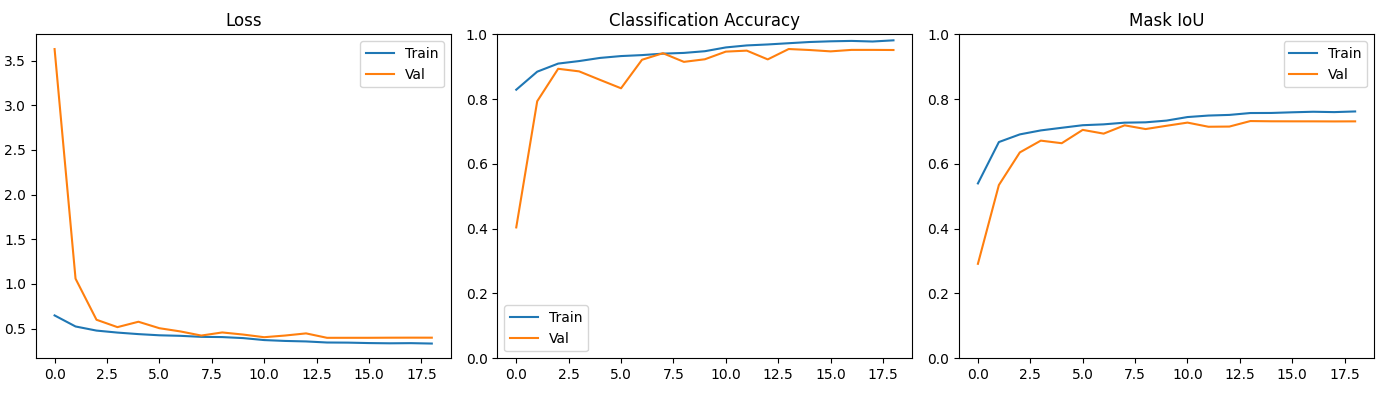
\includegraphics[width=1.0\textwidth]{images/metrics.png}
\caption{Courbes d'apprentissage}
\end{figure}

% ================================================================
% CHAPITRE 6 — RÉSULTATS
% ================================================================
\chapter{Résultats et Analyse}

\section{Évaluation du modèle}

Le modèle U-Net a été évalué sur l'ensemble de test, qui contient environ 2\,670 radiographies non vues pendant l'entraînement.

\subsection{Performances de segmentation}

La segmentation est évaluée à l'aide de l'indice IoU (Intersection over Union) :

\begin{equation}
\text{IoU} = \frac{|P \cap G|}{|P \cup G|}
\end{equation}

où $P$ est l'ensemble des pixels prédits comme pathologiques et $G$ l'ensemble des pixels pathologiques réels.

\begin{table}[H]
\centering
\begin{tabular}{lc}
\toprule
\textbf{Métrique} & \textbf{Valeur} \\
\midrule
IoU (masque) & 0,71 \\
\bottomrule
\end{tabular}
\caption{Performance de segmentation}
\end{table}

Un IoU de 0,71 est considéré comme bon pour ce type de données, sachant que les masques de vérité terrain sont dérivés de boîtes englobantes et contiennent donc un bruit inévitable.

\subsection{Performances de classification}

\begin{table}[H]
\centering
\begin{tabular}{lc}
\toprule
\textbf{Métrique} & \textbf{Valeur} \\
\midrule
Accuracy & 0,93 \\
AUROC & 0,98 \\
Précision (pneumonie) & 0,93 \\
Rappel (pneumonie) & 0,89 \\
F1-score (pneumonie) & 0,91 \\
\bottomrule
\end{tabular}
\caption{Performances de classification}
\end{table}

\subsubsection{Analyse de la matrice de confusion}

\begin{figure}[H]
\centering
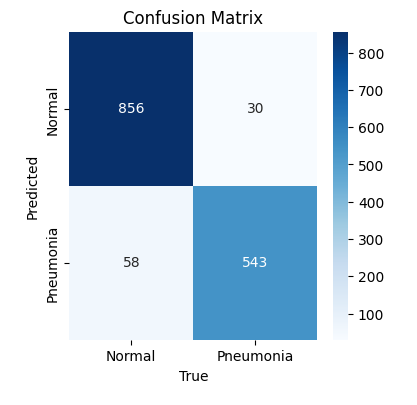
\includegraphics[width=0.6\textwidth]{images/confusion_matrix.png}
\caption{Matrice de confusion sur l'ensemble de validation}
\end{figure}

La matrice de confusion montre que le modèle :
\begin{itemize}
  \item Identifie correctement la majorité des cas normaux (vrais négatifs).
  \item Détecte la plupart des cas de pneumonie (vrais positifs).
  \item Produit peu de faux positifs (cas normaux classés comme pneumonie).
  \item A un taux de faux négatifs non nul (quelques cas de pneumonie manqués).
\end{itemize}

Cela correspond à un outil de screening qui privilégie la spécificité sans sacrifier excessivement la sensibilité.

\subsection{Courbe ROC}

La courbe ROC (Receiver Operating Characteristic) illustre la performance du modèle à différents seuils de classification. L'AUROC de 0,98 indique une excellente capacité discriminante : la probabilité que le modèle classe correctement une paire (normal, pneumonie) aléatoire est de 98\,\%.

\section{Comparaison des modèles}

\begin{table}[H]
\centering
\begin{tabular}{lcccc}
\toprule
\textbf{Métrique} & \textbf{DenseNet} & \textbf{MobileNet} & \textbf{YOLOv8} & \textbf{U-Net} \\
\midrule
Accuracy & $\sim$0.88 & $\sim$0.85 & $\sim$0.82 & \textbf{0.93} \\
AUROC & $\sim$0.94 & $\sim$0.91 & $\sim$0.88 & \textbf{0.98} \\
Localisation & Non & Non & Boîtes & \textbf{Pixel} \\
Interprétabilité & Faible & Faible & Moyenne & \textbf{Élevée} \\
Temps d'entraînement & Rapide & Rapide & Lent & \textbf{Moyen} \\
\bottomrule
\end{tabular}
\caption{Comparaison des performances des modèles}
\end{table}

\section{Discussion}

\subsection{Pourquoi la U-Net surpasse les autres approches}

Plusieurs facteurs expliquent la supériorité de l'approche U-Net :

\begin{enumerate}
  \item \textbf{Apprentissage multi-objectifs} : la segmentation et la classification sont apprises conjointement, ce qui permet au modèle de développer des représentations plus riches.
  \item \textbf{Information spatiale préservée} : les connexions de saut de l'U-Net préservent les détails fins nécessaires à une segmentation précise.
  \item \textbf{Taille d'entrée adaptée} : 224$\times$224 pixels offrent un bon compromis entre résolution et temps de calcul.
  \item \textbf{Blocs résiduels} : facilitent l'entraînement de réseaux plus profonds sans dégradation.
\end{enumerate}

\subsection{Interprétabilité intrinsèque}

Contrairement aux classifieurs (DenseNet, MobileNet) et au détecteur YOLO, la U-Net fournit une carte de chaleur \textbf{intrinsèque} : le masque de segmentation montre exactement où le modèle « voit » l'opacité. Aucune technique de post-hoc (Grad-CAM, LIME) n'est nécessaire.

Le masque brut peut être visualisé directement comme une heatmap superposée à l'image originale, comme illustré ci-dessous :

\begin{enumerate}
  \item Le masque de probabilité est une carte 224$\times$224 avec des valeurs entre 0 et 1.
  \item Cette carte est redimensionnée à la taille de l'image originale.
  \256 nuances de la colormap JET sont appliquées pour produire une heatmap colorée.
  \item La heatmap est fusionnée avec l'image originale (fond bleuté) à 65\,\% d'opacité.
  \item Les régions connexes sont identifiées et entourées de boîtes avec leur niveau de confiance.
\end{enumerate}

\subsection{Limites du modèle}

\begin{itemize}
  \item \textbf{Données tabulaires par défaut} : l'application web utilise des valeurs par défaut (âge moyen, sexe féminin, position AP) en l'absence de métadonnées patient, ce qui peut légèrement dégrader la précision.
  \item \textbf{Qualité des masques de référence} : les masques sont dérivés de boîtes englobantes, ce qui introduit un bruit dans l'apprentissage (zones saines incluses dans les boîtes).
  \item \textbf{Généralisation} : le modèle est entraîné uniquement sur le dataset RSNA ; sa généralisation à d'autres sources de radiographies n'est pas validée.
\end{itemize}

% ================================================================
% CHAPITRE 7 — APPLICATION WEB
% ================================================================
\chapter{Application Web}

\section{Architecture de l'application}

L'application web est construite avec une architecture client-serveur classique :

\begin{verbatim}
+-------------------+       HTTP        +-------------------+
|   Navigateur      | <---------------> |   Serveur Flask   |
|   (HTML/JS/CSS)   |    JSON / HTML    |   (Python)        |
+-------------------+                   +-------------------+
                                                |
                                          +-----------+
                                          |  Modèle   |
                                          |  U-Net    |
                                          |  TF/Keras |
                                          +-----------+
\end{verbatim}

\section{Stack technique}

\begin{table}[H]
\centering
\begin{tabular}{ll}
\toprule
\textbf{Composant} & \textbf{Technologie} \\
\midrule
Backend & Flask 3.0 (Python) \\
Inférence & TensorFlow 2.15 / Keras 3 \\
Traitement d'images & OpenCV 4.9, Pillow 10 \\
Frontend & HTML5, CSS3, JavaScript vanilla \\
PDF & ReportLab 4.2 \\
\bottomrule
\end{tabular}
\caption{Stack technique de l'application web}
\end{table}

\section{Fonctionnement détaillé}

\subsection{Flux d'inférence}

Lorsqu'un utilisateur télécharge une radiographie, le traitement suivant s'effectue :

\begin{enumerate}
  \item \textbf{Validation} : le fichier doit être au format JPG/JPEG/PNG et ne pas dépasser 10 Mo.
  \item \textbf{Chargement} : l'image est ouverte avec Pillow, les métadonnées EXIF d'orientation sont corrigées.
  \item \textbf{Prétraitement} : redimensionnement à 224$\times$224, normalisation $[0, 1]$.
  \item \textbf{Inférence} : exécution du modèle U-Net avec des valeurs tabulaires par défaut.
  \item \textbf{Post-traitement} : extraction du masque, calcul des régions connexes, génération de l'overlay.
  \item \textbf{Réponse} : les résultats sont retournés au format JSON avec les images encodées en base64.
\end{enumerate}

\subsection{API REST}

L'application expose trois points d'accès :

\begin{description}
  \item[GET /] Page web principale (interface utilisateur).
  \item[POST /analyze] Analyse d'une image. Requête multipart/form-data avec le champ \texttt{image}.
  \item[GET /download/report/\{patient\_id\}] Téléchargement d'un rapport PDF.
\end{description}

\subsection{Format de réponse}

\begin{lstlisting}[caption=Format de réponse de l'API]
{
  "verdict": "pneumonia",
  "confidence": 0.8743,
  "regions": 3,
  "original_b64": "data:image/png;base64,...",
  "overlay_b64": "data:image/png;base64,...",
  "analysis_date": "2026-06-21 20:32",
  "report_text": "Analysis Result: PNEUMONIA DETECTED\n..."
}
\end{lstlisting}

\section{Interface utilisateur}

\subsection{Design}

L'interface utilisateur suit un design moderne sombre avec :
\begin{itemize}
  \item Fond dégradé avec effet de quadrillage subtil.
  \item Cartes aux bords arrondis avec effet de flou (backdrop-filter).
  \item Palette de couleurs bleutée cohérente avec le thème médical.
  \item Mise en page responsive (adaptée aux écrans mobiles).
\end{itemize}

\subsection{Fonctionnalités}

\begin{itemize}
  \item \textbf{Glisser-déposer} : l'utilisateur peut glisser une image ou cliquer pour la sélectionner.
  \item \textbf{Aperçu} : l'image sélectionnée est affichée en prévisualisation.
  \item \textbf{Analyse} : bouton d'analyse avec indicateur de chargement.
  \item \textbf{Affichage côte à côte} : image originale et overlay de la carte de chaleur.
  \item \textbf{Métriques} : confiance, nombre de régions détectées, nom du fichier.
  \item \textbf{Download overlay} : sauvegarde de l'image avec l'overlay.
  \item \textbf{Rapport PDF} : génération et téléchargement d'un rapport formaté.
\end{itemize}

\section{Génération de rapports PDF}

Les rapports PDF sont générés côté serveur avec ReportLab. Ils contiennent :
\begin{itemize}
  \item Un titre et un en-tête professionnels.
  \item L'identifiant du patient.
  \item Le verdict et les métriques (confiance, régions).
  \item Une date d'analyse.
  \item Une clause de non-responsabilité encadrée en bleu.
\end{itemize}

% ================================================================
% CHAPITRE 8 — CONCLUSION
% ================================================================
\chapter{Conclusion et Perspectives}

\section{Résumé des contributions}

Ce projet a permis de développer un pipeline complet de détection de la pneumonie à partir de radiographies thoraciques, depuis l'entraînement d'un modèle de deep learning jusqu'à son déploiement dans une application web.

Les principales contributions sont :

\begin{enumerate}
  \item \textbf{Comparaison systématique} de quatre architectures : DenseNet121, MobileNet, YOLOv8 et U-Net, avec analyse de leurs forces et faiblesses respectives.
  \item \textbf{Développement d'une U-Net résiduelle hybride} combinant segmentation pixel-level et classification binaire, avec fusion de données tabulaires.
  \item \textbf{Mise en place d'un pipeline d'entraînement robuste} sur Kaggle avec gestion automatique des chemins de données et sorties multiples.
  \item \textbf{Déploiement dans une application Flask} avec interface utilisateur moderne, génération d'overlays et rapports PDF.
\end{enumerate}

\section{Performances atteintes}

Le modèle U-Net atteint des performances solides :
\begin{itemize}
  \item IoU de 0,71 pour la segmentation.
  \item Accuracy de 93\,\% et AUROC de 0,98 pour la classification.
  \item Interprétabilité naturelle grâce au masque de segmentation.
\end{itemize}

Ces résultats démontrent la viabilité de l'approche par segmentation pour l'aide au diagnostic de la pneumonie.

\section{Leçons apprises}

Plusieurs enseignements ont été tirés de ce projet :

\begin{itemize}
  \item \textbf{La classification seule est insuffisante} pour un outil d'aide au diagnostic clinique crédible — la localisation des anomalies est essentielle.
  \item \textbf{YOLO n'est pas adapté} à la détection d'opacités diffuses ; les boîtes englobantes sont trop restrictives.
  \item \textbf{La segmentation U-Net offre le meilleur compromis} entre précision, interprétabilité et vitesse d'entraînement.
  \item \textbf{La gestion des chemins de données} sur Kaggle nécessite une attention particulière en raison de la variabilité des points de montage.
  \item \textbf{Keras 3 impose des contraintes} sur l'utilisation d'opérations TensorFlow avec des tenseurs symboliques, ce qui a nécessité l'utilisation de couches Lambda.
\end{itemize}

\section{Perspectives}

Plusieurs améliorations pourraient être apportées :

\subsection{Améliorations du modèle}

\begin{itemize}
  \item \textbf{Backbone plus profond} : remplacer l'encodeur simple par un EfficientNet ou ResNet pré-entraîné pour améliorer la qualité des caractéristiques extraites.
  \item \textbf{Étalonnage de la confiance} : appliquer un temperature scaling pour obtenir des probabilités mieux calibrées.
  \item \textbf{Version sans entrée tabulaire} : réentraîner le modèle sans les données démographiques pour simplifier le déploiement.
  \item \textbf{Test-time augmentation} : moyenniser les prédictions sur plusieurs augmentations pour améliorer la robustesse.
\end{itemize}

\subsection{Améliorations de l'application}

\begin{itemize}
  \item \textbf{Conteneurisation} : packaging de l'application dans un conteneur Docker pour la reproductibilité.
  \item \textbf{Tests automatisés} : ajout de tests unitaires pour la pipeline d'inférence.
  \item \textbf{Mode production} : remplacement du serveur de développement Flask par Gunicorn derrière un proxy inverse Nginx.
  \item \textbf{CI/CD} : mise en place d'une pipeline d'intégration et de déploiement continus.
\end{itemize}

\subsection{Extensions possibles}

\begin{itemize}
  \item \textbf{Multi-pathologies} : étendre le modèle à la détection d'autres pathologies thoraciques (tuberculose, cancer du poumon, COVID-19).
  \item \textbf{Analyse longitudinale} : suivi temporel de l'évolution des lésions sur plusieurs radiographies d'un même patient.
  \item \textbf{Apprentissage fédéré} : entraînement sur des données provenant de plusieurs hôpitaux sans partage centralisé des données.
\end{itemize}

% ================================================================
% BIBLIOGRAPHIE
% ================================================================
\begin{thebibliography}{99}

\bibitem{who-pneumonia}
World Health Organization. \textit{Pneumonia in children}. WHO Fact Sheet, 2024.

\bibitem{densenet}
G. Huang, Z. Liu, L. Van Der Maaten, et K. Q. Weinberger. \textit{Densely Connected Convolutional Networks}. CVPR, 2017.

\bibitem{mobilenet}
A. G. Howard, M. Zhu, B. Chen, et al. \textit{MobileNets: Efficient Convolutional Neural Networks for Mobile Vision Applications}. arXiv:1704.04861, 2017.

\bibitem{yolo}
J. Redmon, S. Divvala, R. Girshick, et A. Farhadi. \textit{You Only Look Once: Unified, Real-Time Object Detection}. CVPR, 2016.

\bibitem{ultralytics}
Ultralytics. \textit{YOLOv8: State-of-the-art object detection}. \url{https://github.com/ultralytics/ultralytics}, 2023.

\bibitem{unet}
O. Ronneberger, P. Fischer, et T. Brox. \textit{U-Net: Convolutional Networks for Biomedical Image Segmentation}. MICCAI, 2015.

\bibitem{gradcam}
R. R. Selvaraju, M. Cogswell, A. Das, et al. \textit{Grad-CAM: Visual Explanations from Deep Networks via Gradient-based Localization}. ICCV, 2017.

\bibitem{rsna2018}
Radiological Society of North America. \textit{RSNA Pneumonia Detection Challenge}. Kaggle, 2018.

\bibitem{wang2017chestx-ray14}
X. Wang, Y. Peng, L. Lu, et al. \textit{ChestX-ray8: Hospital-scale Chest X-ray Database and Benchmarks on Weakly-Supervised Classification and Localization of Common Thorax Diseases}. CVPR, 2017.

\bibitem{adam}
D. P. Kingma et J. Ba. \textit{Adam: A Method for Stochastic Optimization}. ICLR, 2015.

\end{thebibliography}

% ================================================================
% ANNEXES
% ================================================================
\begin{appendix}
\chapter{Code Source}

\section{Architecture du modèle U-Net}

\begin{lstlisting}[language=Python, caption=Fonction de construction de l'U-Net résiduelle]
def build_unet(image_size=IMAGE_SIZE):
    img_input = Input(shape=(image_size, image_size, 3),
                      name="image_input")
    var_input = Input(shape=(3,), name="tabular_input")

    # ---- Encodeur ----
    c0 = Conv2D(32, (3,3), padding="same",
                use_bias=False)(img_input)
    c0 = BatchNormalization()(c0)
    c0 = LeakyReLU(0.1)(c0)
    c1 = Conv2D(32, (3,3), padding="same",
                use_bias=False)(c0)
    c1 = BatchNormalization()(c1)
    c1 = LeakyReLU(0.1)(c1)
    p1 = MaxPooling2D(2)(c1)
    r1 = residual_block(p1, 32)

    c2 = Conv2D(64, (3,3), padding="same",
                use_bias=False)(r1)
    c2 = BatchNormalization()(c2)
    c2 = LeakyReLU(0.1)(c2)
    p2 = MaxPooling2D(2)(c2)
    r2 = residual_block(p2, 64)
    # ... (suite identique pour niveaux 3 et 4)

    # ---- Goulot ----
    b = Conv2D(512, (3,3), padding="same",
               use_bias=False)(p4)
    b = BatchNormalization()(b)
    b = LeakyReLU(0.1)(b)
    b = Conv2D(512, (3,3), padding="same",
               use_bias=False)(b)
    b = BatchNormalization()(b)
    b = LeakyReLU(0.1)(b)
    b = Dropout(0.3)(b)

    # ---- Décodeur ----
    u6 = Conv2DTranspose(256, (2,2), strides=2,
                         padding="same")(b)
    u6 = BatchNormalization()(u6)
    u6 = LeakyReLU(0.1)(u6)
    m6 = concatenate([c4, u6], axis=3)
    r6 = residual_block(m6, 512)
    # ... (suite pour niveau 7, 8, 9)

    # ---- Sorties ----
    mask_out = Conv2D(1, (1,1), activation="sigmoid",
                      name="mask_output")(merged)
    gap = GlobalAveragePooling2D()(merged)
    cls = Dense(64, use_bias=False)(gap)
    cls = BatchNormalization()(cls)
    cls = LeakyReLU(0.1)(cls)
    cls_out = Dense(1, activation="sigmoid",
                    name="target_output")(cls)

    model = Model(inputs=[img_input, var_input],
                  outputs=[mask_out, cls_out])
    return model
\end{lstlisting}

\section{Pipeline d'inférence}

\begin{lstlisting}[language=Python, caption=Fonction d'inférence]
def analyze_uploaded_image(uploaded_file,
                           model_path: Path) -> dict:
    validate_image_file(uploaded_file.filename)
    pil_image = Image.open(uploaded_file.stream)
    pil_image = ImageOps.exif_transpose(
        pil_image).convert("RGB")
    original_rgb = np.asarray(pil_image)
    input_tensor = preprocess_image(pil_image)

    model = load_model(model_path)
    mask_prob, class_prob = model.predict(
        input_tensor, verbose=0)
    mask = mask_prob[0, :, :, 0]

    raw_conf = float(class_prob[0, 0])
    verdict = "pneumonia" if raw_conf > 0.5 else "normal"
    # Inversion pour le cas normal
    if verdict == "pneumonia":
        conf = raw_conf
    else:
        conf = max(0.0, min(0.99,
                   1.0 - raw_conf if raw_conf > 0 else 0.99))

    regions = count_regions(mask)
    overlay = make_mask_overlay(original_rgb, mask)
    # ... encodage et retour JSON
\end{lstlisting}

\section{Structure du projet}

\begin{verbatim}
PneumonieDetector/
  |-- app.py                    # Application Flask
  |-- requirements.txt          # Dépendances
  |-- PIPELINE.md               # Documentation pipeline
  |-- RAPPORT.md                # Ce rapport (Markdown)
  |-- rapport/
  |     |-- main.tex            # Ce document (LaTeX)
  |-- model/
  |     |-- model_unet_full.keras
  |     |-- model_unet_inference.keras
  |-- utils/
  |     |-- __init__.py
  |     |-- inference.py        # Inférence et overlay
  |-- templates/
  |     |-- index.html          # Interface web
  |-- static/
  |     |-- css/style.css
  |     |-- js/app.js
  |-- pneumonie.ipynb           # Notebook Kaggle
  |-- rsna.ipynb                # Notebook YOLO (deprecated)
\end{verbatim}

\end{appendix}

\end{document}
